\documentclass[12pt,fleqn]{article}
\usepackage{jp-report} % loads the JP Report formatting
% Add any package, do it here:

\let\oldverbatim\verbatim
\let\oldendverbatim\endverbatim
\renewenvironment{verbatim}{\endgraf\footnotesize\singlespace\oldverbatim}{\oldendverbatim\endsinglespace}

% Start of the document
\begin{document}

%%%%%%%%TITLE PAGE with TOC%%%%%%%%%%%%%%%%%%%%%%%%%%%%

\title{How to Efficiently Turn Your Paper into a Joint Program Report:\protect\\
  The JP \LaTeX\, Template Version 1.3}

\author{Erwan Monier%
\thanks{Author affiliation should go here, \textit{e.g.}, Joint Program of the
  Science and Policy of Global Change, Massachusetts Institute of Technology,
  Cambridge, MA. \textit{This is Version 1.2 of this guide, last udated May 24,
  2012}.}
\thanks{Corresponding author (Email:
  \href{mailto:emonier@mit.edu}{emonier@mit.edu})}~
and
Sebastian Rausch\thanksmark{1}
}

\maketitle % Automatically creates the title and author informations (do not remove)

\begin{abstract}
This note documents version 1.2 of the JP \LaTeX\, template for
creating papers submitted to the MIT Joint Program Report Series. This template
provides an efficient and rapid way to produce a JP Report that is consistent
with current formatting guidelines. It manages the entire layout and format
parameters of your document including the title page, abstract, section
headings, figure and table captions, footnotes, acknowledgements, appendices,
and the bibliography. All files required to generate this document are available
on the JP Wiki webpage.
\end{abstract}

\begin{singlespace}
\tableofcontents % Automatically creates the Table of Contents (do not remove)
\end{singlespace}

\section{Introduction}

This note documents version 1.2 of the JP \LaTeX\, template that provides an
efficient and rapid way to turn your research paper into a JP Report. This
template formats your document to be consistent with the official formatting
guidelines of the MIT Joint Program Report Series. Most importantly, it frees up
additional research time by avoiding resource-intensive battles with MS-Word.
This template is based on the word processing software \LaTeX, which is open
source software; the latest version of the JP \LaTeX\, template is available
online at the JP Wiki page.

This note is primarily concerned with providing an alternative option to format
your JP Report. As such, it should be seen as complementing the existing MS-Word
JP template document ``\emph{JP Report Preparation Guidelines for Authors}'' by
Anne Slinn and Gwendolyn Kelso. The remainder of this document showcases the
\LaTeX\, template and provides a brief description of how to implement this new
package. If there are suggestions for how to improve the usefulness or accuracy
of this template, or the accompanying template document, please email comments
to the authors of this note.

\section{File Structure of the JP \LaTeX\, Package}

The JP \LaTeX\, package can be found on the JP Wiki Report Series Information 
webpage. It consists of the following files: 
\begin{description}
  \item[\ttfamily jp-report.sty] controls all formatting and layout
  parameters. Do not modify this file and keep it in the same directory as your
  JP report!
  \item[\ttfamily template.tex] This is the core file
  that was used to create the PDF file called \textit{JP\_Report\_template.pdf}
  that you are currently reading. You can use it as a template by inserting the
  text of your report. 
  \item[\ttfamily example.bib] This file contains the bibliography
  items used in this document and serves as a template for your JP report
  bibliography. This file should be stored in the same directory as your JP
  report. You can add references here following the format described in the
  bibliography section of this document.
  \item[\ttfamily jpreport.bst] defines the style of the bibliography. Do not
  modify this file and keep it in the same directory as your JP report!
\end{description}

\section{Submission Guidelines}
Joint Program Reports are usually required to be authored (or co-authored) by
personnel affiliated with the Joint Program. The content is generally expected
to be an article that has been prepared for submission to a peer-reviewed outlet
(journal or book chapter).

The general procedure for contributing a paper to the Report Series is the
following:
\begin{enumerate}
  \item Authors should first confer with John Reilly (Policy/Economics) or Anne
  Slinn (Science) to determine if the paper is suitable to be included in the
  Report Series.
  \item If given the ``go-ahead'', authors prepare their paper for production 
  according to the guidelines in this document. Authors are individually 
  responsible for the proper formatting and editing of their papers.
  \item The author will then email the ``print-ready'' paper as a PDF file to 
  Fran Goldstein (\href{mailto:fkg@mit.edu}{fkg@mit.edu}) for format review. 
  The paper must be delivered in PDF format. \LaTeX\, allows you to directly 
  create a PDF document from the source code. Please ensure that all graphics 
  in the PDF document are sharp and clear images. (The process of saving as, or 
  converting to, a PDF file may involve option-settings that can default to 
  `down-sampling' graphics, which reduces image quality/resolution to reduce 
  file-size.) If the paper meets all formatting criteria, it will go into the 
  production process.
  \item If the paper does not match the formatting criteria (unlikely to be the 
  case if you use this new template \emph{without} modifying it, and if you 
  know how to use \LaTeX), it will be sent back to the author for correction 
  (may take several rounds).
\end{enumerate}

\section{Basic Functionalities of the JP \LaTeX\, Package}

\subsection{Headings}

To do a section, subsection, or subsubsection heading, simply type:
\begin{verbatim}
\section{Headings}
\subsection{Headings}
\subsection{Headings}
\end{verbatim}
The format of the headings (font size, capitalization, font type, numbering, 
spacing before and after the heading etc.) is controlled by the template.

\subsubsection{Paragraph Attributes}

A new paragraph is specified by typing:
\begin{verbatim}
\par
\end{verbatim}
\ldots or simply by leaving a blank line between two blocks of text:
\begin{verbatim}
Here is one sentence.
Here is a second sentence, part of the same paragraph.

This sentence appears in a new paragraph.
\end{verbatim}

\subsection{Specific Sections}

\subsubsection{Title Page}

The whole title page including the title of the paper, the author list, 
abstract, and table of contents is created automatically. Simply insert the 
information in the respective customized fields:
\begin{verbatim}
\title{}
\author{}
\affil{}
\abstract{}
\end{verbatim}

\subsubsection{Table of Contents}

The table of contents together with the page numbers is generated automatically 
from the section headings included in the document by the command 
\verb@\tableofcontents@. Do not remove that command from the template.

\subsubsection{Tables}

An example how to generate the following \textbf{Table \ref{table:topdown_var}} 
can be found in the source code. To reference a table the command is as 
follows. First, create a label for the table as in:
\begin{verbatim}
\label{table:label}
\end{verbatim}
Then any reference to this table can be made by:
\begin{verbatim}
Table \ref{table:label}
\end{verbatim}.
Boldface the first reference to a table in the text by using the command 
\begin{verbatim}
\textbf{Table \ref{table:label}}
\end{verbatim}

\begin{table}[h]
\caption{Regional Price Elasticities for Fuel Supply and Electricity Demand.}
\label{table:elas_bernstein}
\small\centering
\begin{tabularx}{\linewidth}{%
  X % this is to specific automatic column width
  S[table-format=1.2]% Define the format of the numbers in the column 
  S[table-format=1.2]% This allows for decimal point alignment
  S[table-format=1.2]%
  S[table-format=1.2]%
  }
  \toprule
  \tableheader{1}{L}{Region} &
    \tableheader{2}{c}{$\eta^z_r$ (simulated)$\,^a$} &
    \tableheader{1}{C}{$\epsilon_r$ (simulated)$\,^a$} &
    \tableheader{1}{C}{$\epsilon_r$ (estimated)} \\
% use \tableheader to input the headers of the columns as such:
% \tableheader{#column}{alignment}{text}
% where
% #column is 1 unless using multicolumn header like in this example;
% alignment is either: L, C or R for (left align, centered, right align). Note 
% that if #column is greater than 1, you should use l, c or r in lowercase;
% text is the header text (it will automatically be bolded).
  \cmidrule{2-3} &
    \tableheader{1}{C}{Coal} &
    \tableheader{1}{C}{Natural gas} & & \\
  \midrule
  CA    & 0.01 & 0.02 & -50.47 & -0.25 \\
  ERCOT & 0.01 & 0.04 & -0.435 & -0.15 \\
  MISO  & 0.03 & 0.01 & -0.24  & -0.14 \\
  MOUNT & 0.01 & 0.02 & -0.37  & -0.20 \\
  NENGL & 0.01 & 0.01 & -0.72  & -0.19 \\
  NWPP  & 0.09 & 0.01 & -0.43  & -0.23 \\
  NY    & 0.01 & 0.01 & -0.17  & -0.10 \\
  PJM   & 0.04 & 0.01 & -0.23  & -0.22 \\
  SEAST & 0.05 & 0.01 & -0.32  & -0.25 \\
  SPP   & 0.01 & 0.01 & -0.50  & -0.15 \\
  \bottomrule
\end{tabularx}
\end{table}

\subsubsection{Figures}

An example how to generate the following \textbf{Figure 
\ref{fig:mapregionalaggregation}} can be found in the source code. To reference 
a figure the command is as follows. First, create a label for the figure as in:
\begin{verbatim}
\label{fig:label_name}
\end{verbatim}
Then any reference to this table can be made by:
\begin{verbatim}
Figure \ref{fig:label_name}
\end{verbatim}.
Boldface the first reference to a figure in the text by using the command:
\begin{verbatim}
\textbf{Figure \ref{fig:label_name}}
\end{verbatim}.

\begin{figure}[h]
  \centering
  \noindent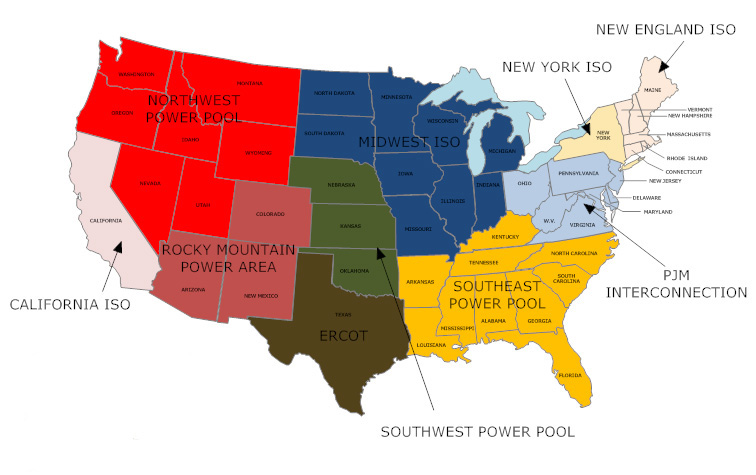
\includegraphics[width=13cm]{MapUS12.jpg}\\
  \caption{U.S. Regions in Integrated Economic-Electricity Model.}\label{fig:mapregionalaggregation}
\end{figure}

\subsubsection{Equations}

Creating equations in \LaTeX\, is simple. You can find the \LaTeX\, coding following equations in the source code of this document:
\begin{equation}\label{eq1}
\text{ELE}^{\text{F}}_r + \sum_{\text{NF}} \text{ELE}^{\text{NF}}_r = \text{D}^{\text{ELE}}_r \quad \perp \quad P^{\text{ELE}}_r
\end{equation}
\begin{equation}\label{eq2}
\frac{\partial \overline{u}}{\partial t}=f\overline{v}^\star-\frac{\overline{v}^\star}{a\cos \phi} \frac{\partial}{\partial \phi} \left(\overline{u} \cos \phi \right)-\overline{w}^\star \overline{u}_{z}+\frac{1}{\rho_{0} a \cos \phi}\nabla\cdot\vec{F}+\overline{X}
\end{equation}
For more details on the full functionality of the math package go and read the documentation at: \url{ftp://ftp.ams.org/pub/tex/doc/amsmath/amsldoc.pdf}.


\subsubsection{Footnotes}

To do footnotes,\footnote{This is footnote text. This is footnote text.} simply
type:
\begin{verbatim}
\footnote{This is footnote text This is footnote text.}
\end{verbatim}

\subsubsection{Acknowlegments}

The acknowledgments go right before the bibliography using the following command:
\begin{verbatim}
\acknowledgments{}
\end{verbatim}

\subsubsection{Bibliography}

You can store your bibliography in BibTeX format and call it using the 
following command, which should be placed after the acknowledgments but before 
the appendices:
\begin{verbatim}
\bibliography{name_of_bibliography_file}
\end{verbatim}

The reference is then cited using the commands {\footnotesize\verb|\citet|} and 
{\footnotesize\verb|\citep|} for textual and parenthetical citations, 
respectively:

\bigskip

\noindent{\footnotesize\verb|\citet{Reilly2007}|} produces: \citet{Reilly2007}\\
\noindent{\footnotesize\verb|\citep{Webster2003}|} produces: \citep{Webster2003}

\bigskip

Example bibliography entries for the various types of references are given 
below. The full bibliography database can be found in the 
\textit{template\_bibliography.bib} file located in the JP \LaTeX\, template 
package. Last, the resultant formatted references are given at the end of this 
document in the references section. Authors should use the example database 
entry to determine what information is necessary to have a properly formatted 
reference in JP report style. 

\begin{itemize}
\item Journal article:
\end{itemize}
\begin{verbatim}
@ARTICLE{Bugnion2006,
  AUTHOR = {Bugnion, V. and C. Hill and P. H. Stone},
  YEAR = {2006},
  TITLE = {An Adjoint Analysis of the Meridional Overturning Circulation in a
  Hybrid Coupled Model},
  JOURNAL = {Journal of Climate},
  VOLUME = {19},
  NUMBER = {15},
  PAGES = {3751-3767}}
\end{verbatim}

\begin{itemize}
\item Journal article with JP reprint:
\end{itemize}
\begin{verbatim}
@REPRINT{Webster2003,
  AUTHOR = {Webster, M. D. and C. E. Forest and J. M. Reilly and M. H. Babiker
  and D. W. Kicklighter and M. Mayer and R. G. Prinn and M. C. Sarofim
  and A. P. Sokolov and P. H. Stone and C. Wang},
  YEAR = {2003},
  TITLE = {Uncertainty Analysis of Climate Change and Policy Response},
  JOURNAL = {Climatic Change},
  VOLUME = {61},
  NUMBER = {3},
  PAGES = {295-320},
  INSTITUTION = {MIT JPSPGC},
  TYPE = {Reprint 2003-11},
  URL = {http://mit.edu/globalchange/www/MITJPSPGC_Reprint03-11.pdf}}
\end{verbatim}

\begin{itemize}
\item Journal article with JP preprint:
\end{itemize}
\begin{verbatim}
@PREPRINT{Babiker2007,
  AUTHOR = {Babiker, M. and R. S. Eckaus},
  YEAR = {2007},
  TITLE = {Unemployment Effects of Climate Policy},
  JOURNAL = {Environmental Science and Policy},
  NOTE = {in press; see also},
  INSTITUTION = {MIT JPSPGC},
  TYPE = {Report 137},
  URL = {http://mit.edu/globalchange/www/MITJPSPGC_Rpt137.pdf}}
\end{verbatim}

\begin{itemize}
\item Journal article submitted/in press without a JP preprint, or article in 
preparation:
\end{itemize}
\begin{verbatim}
@UNPUBLISHED{Gao2007,
  AUTHOR = {Gao, X. and P. A. Dirmeyer and Z. Guo and M. Zhao},
  TITLE = {Sensitivity of Land Surface Simulations to the Treatment of Vegetation
  Properties and the Implications for Seasonal Climate Prediction},
  YEAR = {2008},
  JOURNAL = {Journal of Hydrometeorology},
  NOTE = {submitted}}
\end{verbatim}

%\begin{itemize}
%\item Article in preparation:
%\end{itemize}
%\begin{verbatim}
%@UNPUBLISHED{Schlosser2007,
%	AUTHOR = {Schlosser, C. A. and M. Webster and C. E. Forest},
%	YEAR = {2007},
%	TITLE = {A Probabilistic Description of Global Precipitation-Frequency Change
%	under Climate Warming},
%	NOTE = {Manuscript in preparation}}
%\end{verbatim}

\begin{itemize}
\item Technical Report:
\end{itemize}
\begin{verbatim}
@TECHREPORT{Paltsev2005,
  AUTHOR = {Paltsev, S. and J. Reilly and H. Jacoby and R. Eckaus and
  J. McFarland and M. Babiker},
  YEAR = {2005},
  TITLE = {The MIT Emissions Prediction and Policy Analysis (EPPA) Model:
  Version 4},
  INSTITUTION = {MIT JPSPGC},
  TYPE = {Report 125},
  MONTH = {August},
  PAGES = {72},
  URL = {http://mit.edu/globalchange/www/MITJPSPGC_Rpt125.pdf}}
\end{verbatim}

\begin{itemize}
\item Technical Note:
\end{itemize}
\begin{verbatim}
@TECHREPORT{Gurgel2007b,
  AUTHOR = {Gurgel, A. and G. Metcalf and N. Osouf and J. Reilly},
  YEAR = {2007b},
  TITLE = {Computing Tax Rates for Economic Modeling: A Global Dataset Approach},
  INSTITUTION = {MIT JPSPGC},
  TYPE = {Technical Note 11},
  MONTH = {January},
  PAGES = {13},
  URL = {http://mit.edu/globalchange/www/MITJPSPGC_TechNote11.pdf}}
\end{verbatim}

\begin{itemize}
\item Dissertation/Thesis:
\end{itemize}
\begin{verbatim}
@THESIS{Sugiyama2007,
  AUTHOR = {Sugiyama, M.},
  YEAR = {2007},
  TITLE = {Estimating the Economic Cost of Sea-Level Rise},
  TYPE = {Master of Science Thesis in Technology and Policy},
  SCHOOL = {Massachusetts Institute of Technology},
  ADDRESS = {Cambridge, MA}}
\end{verbatim}

\begin{itemize}
\item Book edited:
\end{itemize}
\begin{verbatim}
@BOOK{Ellerman2007,
  EDITOR = {Ellerman, A.D. and B. Buchner and C. Carraro},
  YEAR = {2007},
  TITLE = {Allocation in the European Emissions Trading Scheme: Rights, Rents,
  and Fairness},
  PUBLISHER = {Cambridge University Press},
  ADDRESS = {Cambridge, UK},
  PAGES = {448}}
\end{verbatim}

\begin{itemize}
\item Book chapter:
\end{itemize}
\begin{verbatim}
@INBOOK{Reilly2007,
  AUTHOR = {Reilly, J. and B. Felzer and D. Kickligher and J. Melillo and H. Tian
  and M. Asadoorian},
  YEAR = {2007},
  TITLE = {The Prospects for Biological Carbon Sinks in Greenhouse Gas Emissions
  Trading Systems},
  BOOKTITLE = {Greenhouse Gas Sinks},
  EDITOR = {Reay, D. and C. N. Hewitt and K. Smith and J. Grace},
  PUBLISHER = {CABI Publishing},
  ADDRESS = {Wallingford, UK},
  CHAPTER = {8},
  PAGES = {115-142}}
\end{verbatim}

\begin{itemize}
\item Book Chapter Forthcoming:
\end{itemize}
\begin{verbatim}
@INBOOK{Jacoby2007,
  AUTHOR = {Jacoby, H.},
  YEAR = {2007},
  TITLE = {Climate Favela: A Comment on Barrett},
  BOOKTITLE = {Architectures for Agreement: Assessing Global Climate Change in
  the Post-Kyoto World},
  EDITOR = {J. Aldy and R. Stavins},
  PUBLISHER = {Cambridge University Press},
  ADDRESS = {Cambridge, UK},
  NOTE = {forthcoming}}
\end{verbatim}

\begin{itemize}
\item Conference Preprints/Proceedings/Extended Abstracts:
\end{itemize}
\begin{verbatim}
@INPROCEEDINGS{Kim2006,
  AUTHOR = {Kim, D. and C. Wang and A. M. Ekman and M. C. Barth and P. J. Rasch},
  YEAR = {2006},
  TITLE = {Climate Impact of Anthropogenic Aerosols in an Interactive
  Size-Resolving Aerosol-Climate Model},
  BOOKTITLE = {Eos Trans.},
  ORGANIZATION = {AGU},
  VOLUME = {87},
  NUMBER = {52},
  NOTE = {{F}all Meeting Supplement, Abstract A33B-0978}}
\end{verbatim}

\subsubsection{Appendices}

The appendix or appendices should follow the references using the command:
\begin{verbatim}
\appendix                             % to start the appendix portion
\appsection{}                         % if the appendix does not have a title
\appsection{: Title of the Appendix}  % if the appendix has a title
\end{verbatim}

Figures and tables inserted in the appendix will automatically be labeled 
according to the appendix number.

\section{Updates from Last Version}

Version 1.2 of the JP \LaTeX\, template includes the following:
\begin{itemize}
  \item Corrected the indentation and hang of footnotes and affiliations;
  \item Corrected the use of ``,'' and ``and'' in the list of authors on the 
  title page;
  \item Corrected the justification of captions.
\end{itemize}
Please contact the authors of this template if you think improvements to this 
template are necessary.

\section{Conclusion}

This is a nice \LaTeX\, template.

\acknowledgments{The acknowledgments immediately follow the main text. It 
should be brief and should only acknowledge those who provided direct help in 
the research and writing of the report. It is also where financial support is 
acknowledged.}

% - \nocite{key} causes the BibTeX item `key' to be included in the
% bibliography, without a citation appearing in the document.
% - \nocite{*} does the same for ALL entries in the .bib file.
\nocite{*}

% Use the JP Report style for items in the bibliography
\bibliographystyle{jpreport}

% Include bibliography items from example.bib
\bibliography{example}

% Begin the appendic
\newpage
\appendix

\appsection{: Greenhouse Gamble Wheels}

This is the appendix A.

\begin{figure}[h!]
  \centering
  \noindent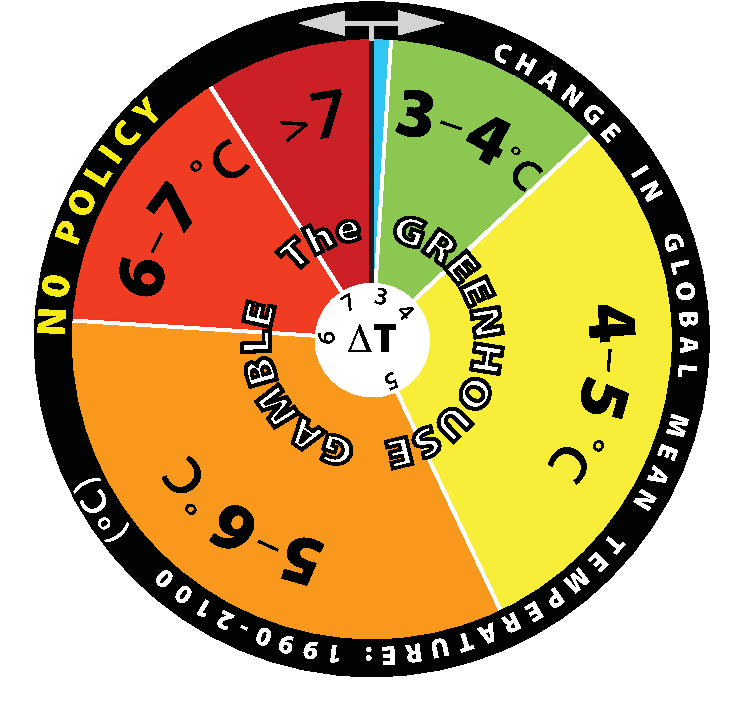
\includegraphics[width=3.6in]{GHG_ReferenceWheel2009.pdf}\\
  \caption{The MIT JP Greenhouse Gamble wheel for the reference case (no policy).}\label{fig:jpwheelnopolicy}
\end{figure}

\begin{figure}[h!]
  \centering
  \noindent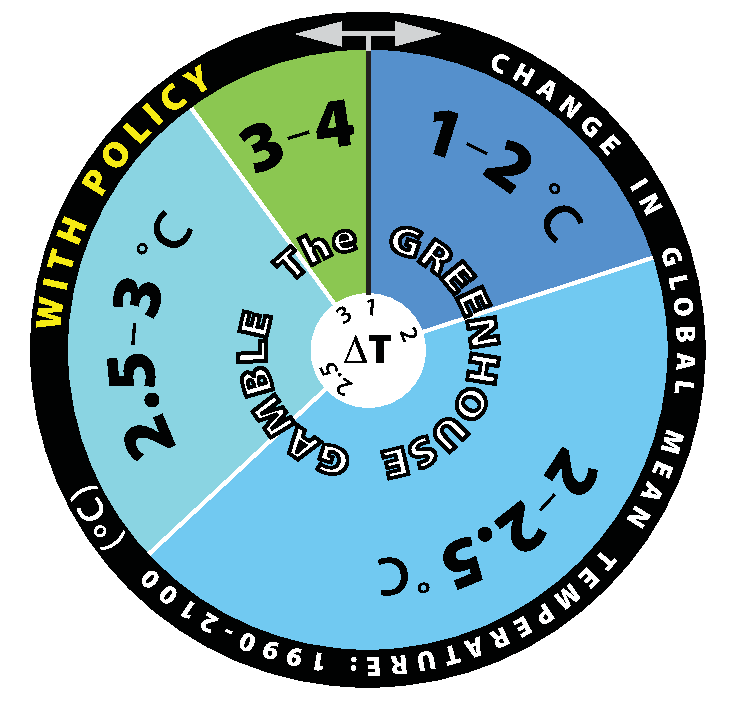
\includegraphics[width=3.6in]{GHG_PolicyWheel2009.pdf}\\
  \caption{The MIT JP Greenhouse Gamble wheel for the policy case (550 ppm CO$_{2}$).}\label{fig:jpwheel550policy}
\end{figure}

\newpage

\appsection{}

This is the appendix B.

\begin{table}[h]
\caption{ Equilibrium Variables Related to Electricity in Top-down Model.}\label{table:topdown_var}
   \small
   \centering
\begin{tabularx}{\textwidth}{>{\hsize=4cm}X X}
% By default, using X as the column type of tabularx spreads the column width evenly. If it is needed to specify the width of a column this can be done using the following format:
% instead of X, use >{\hsize=4cm}X where 4cm can be changed to whatever width is desired.
   \toprule
   \tableheader{2}{l}{\emph{Activity variables}}\\
   \midrule
   $\text{ELE}^{\text{NF}}_r$    &   Electricity generation from technology $\text{NF}$ in $r$\\
   $\text{ELE}^{\text{F}}_r$     &   Electricity generation from fossil fuels in $r$\\
   $\text{ELE}^{\text{NF}}_r$    &   Electricity generation from technology $\text{NF}$ in $r$\\
   $D^{\text{ELE}}_r$            &   Demand for electricity in $r$\\
   $S^i_r$\,,\,$D^i_r$           &   Supply and demand for commodity $i$ in non-electricity sectors in $r$\\
   $L_r\,,\,D^{\text{L}}_r$      &   Labor supply and demand in non-electricity sectors in $r$\\
   $K_r\,,\,D^{\text{K}}_r$      &   Capital supply and demand in non-electricity sectors in $r$\\
   $S^{\text{FUEL}}_r\,,\,D^{\text{FUEL}}_r$      &   Fossil fuel supply and demand in non-electricity sectors in $r$\\
   $S^{\text{NF}}_r$             &   Supply of technology-specific resource in $r$\\
   \midrule
   \tableheader{2}{l}{\emph{Price variables}} \\
   \midrule
   $P^{\text{ELE}}_r$       &   Price index for electricity generation in $r$\\
   $P^{\text{NF}}_r$        &   Price index for technology-specific resource $\text{NF}$  in $r$\\
   $P^{\text{K}}$           &   Rental price for capital \\
   $P^{\text{L}}_r$         &   Wage rate  in $r$\\
   $P^{\text{FUEL}}_r$      &   Price index for fossil fuel $\text{FUEL}$ in $r$\\
   $P^i_r$                  &   Price index non-energy commodity $i$ in $r$\\
      \bottomrule
\end{tabularx}
\end{table}

\begin{figure}[h!]
  \centering
  \noindent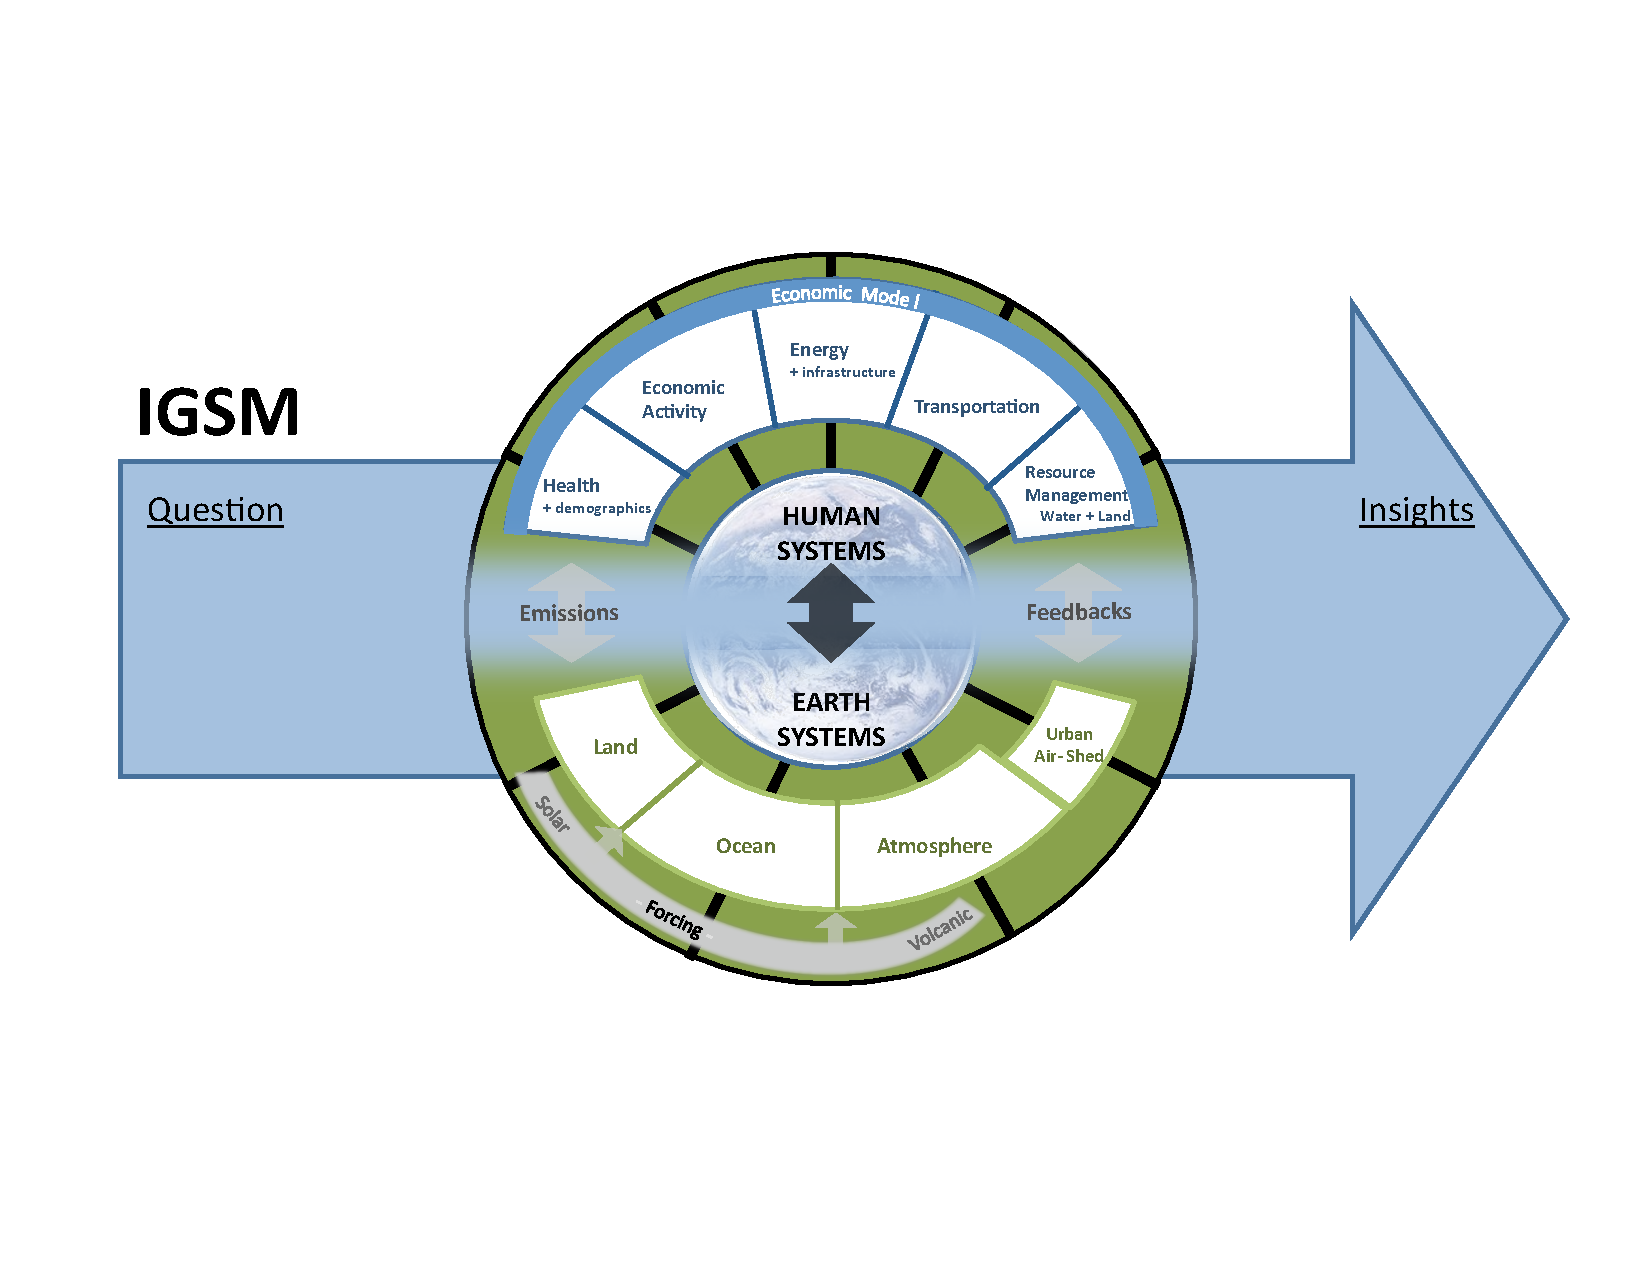
\includegraphics[width=\textwidth]{IGSM_schematic.pdf}
  \caption{Schematic of the MIT Integrated Global System Model framework.}\label{fig:igsmschematic}
\end{figure}

\end{document}
